%!TEX root = ../fbi.tex

\section{Correlation functions}
\label{sec:Correlations}

In Ref.~\onlinecite{kimchi2013}, certain real-space correlation functions
of the featureless boson insulator state were studied using a mapping to
a particular classical statistical mechanical system which was sampled using
Monte Carlo techniques.
Here, we go beyond this by employing PEPS calculations on infinite cylinders
that allow us to measure a broader class of correlation functions and, in
particular, allow us establish a strict upper bound on the exponential decay
of \emph{all} two-point correlation functions for an infinite cylinder of
given width.

\begin{figure}
	\centering
	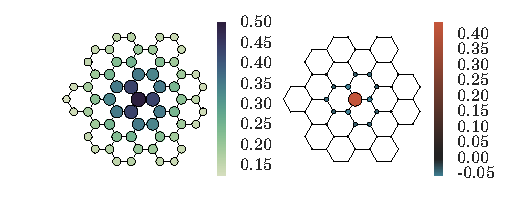
\includegraphics[width=\columnwidth]{ShortDistanceCorrelations_SCB_L8.pdf}
	\vskip-5ex
	\caption{
	 Short distance correlation functions $\ev{b_0^{\dagger} b_x}$ (left panel)
	 and $\ev{(n_0-\frac12)(n_x-\frac12)}$ (right panel) for the soft-core HFBI
	 on the $W=8$ cylinder.
	 The magnitude of the correlation function at site $x$ is proportional to
	 the area of the corresponding circle.
	 \brayden{Put the hardcore case to match the next figure?}
	 }
	\label{fig:ShortCorr}
\end{figure} 

In Fig.~\ref{fig:ShortCorr}, we show both density-density and off-diagonal
short-range correlation functions for a cylinder of circumference $W=8$.
Comparing these to the Monte Carlo results of Ref.~\onlinecite{kimchi2013},
which have been computed for a different geometry, we find good qualitative
agreement. Crucially, while the boundary conditions we choose break the rotational
symmetry by making the system periodic in one direction and infinite in the other,
the short-range correlations for distances up to half of the cylinder circumference
appear unaffected by this.

It is a well-known result that PEPS can, in the thermodynamic limit,
exhibit power-law correlation functions~\cite{verstraete2006}, while the correlation
functions in an MPS of finite bond dimension decay exponentially. The
long-range correlations of an MPS are encoded in its transfer operator $T$,
which for an MPS of bond dimension $M$ is a matrix of size $M^2 \times M^2$.
Denoting the spectrum of $T$ as $\lambda_i$ with $|\lambda_0| \geq |\lambda_1| \geq \ldots$,
we can normalize the state such that $\lambda_0 = 1$. If the largest eigenvalue
is found to be non-degenerate, $\lambda_1 < \lambda_0$, we have that all correlation
functions of operators $\mathcal{O}_i$ that are supported on a finite number of sites centered
around a site $i$ decay as
$\langle \mathcal{O}_i \mathcal{O}_j \rangle - \langle \mathcal{O}_i \rangle \langle \mathcal{O}_j \rangle \sim e^{-|i-j|/\xi_\mathcal{O}}$.
Crucially, the correlation length $\xi_\mathcal{O}$ for any operator $\mathcal{O}$
is bounded from above by $-1/\log |\lambda_1|$~\cite{schollwock2005}.\bela{What to cite here?}
In the following, we thus
evaluate the spectrum of the transfer operator of our PEPS along cylinders of varying
circumference $W$ to establish an upper bound on the correlation length for each
circumference $\xi(W)$
Note that the possibility of having power-law correlations in a PEPS can
be reconciled with the above consideration if the correlation length $\xi(W)$
diverges as $W \rightarrow \infty$; we will thus need to carefully consider the scaling
of $\xi(W)$.

\begin{figure}
	\centering
	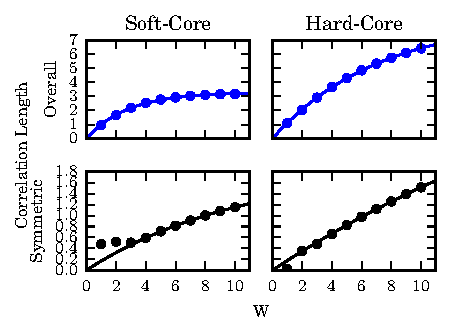
\includegraphics[width=\columnwidth]{CorrelationBounds_fits.pdf}
	\vskip-2em
	\caption{Bound on the correlation length of all operators and $U(1)$ symmetric operators
	 respectively for the soft-core and hard-core states vs. cylinder circumference $W$.
	 Fits of the form $\xi = \xi_{\infty} - Ae^{-W/B}$ were
	 used to extract the correlation lengths.
	 These bounds can be confirmed to match the correlation lengths of 
	 $\ev{b^{\dagger}_x b_y}$ and $\ev{n_x n_y}$ in each case.
	}
	\label{fig:TMS}
\end{figure}

Our results for the correlation bounds $\xi(W)$ are shown in Fig.~\ref{fig:TMS}.
Here, we show the upper bound for the case of soft-core and hard-core bosons,
and in each case consider the spectrum of the full transfer operator as well
as $S^z=0$ sector, which encodes correlations of operators $\mathcal{O}_i$ that do not
change the boson number (such as density-density correlations).
We find that in each case, the largest eigenvalue of the transfer operator is
non-degenerate. Furthermore, we find
that the correlation length approaches a finite constant as we
increase $W$, as shown in Figure \ref{fig:TMS}.
